\section{Appendix: Conceptual Pipeline Design \label{sec:scipi}}

A high-level conceptual overview of the LSST image processing science pipelines is illustrated
in Figure~\ref{fig:Detail1}. 
The pipeline definitions presented here are driven by their inputs,
outputs and processing steps; they do \textit{not} describe exact boundaries in the actual implementation
code, execution, or development responsibilities within the Project.
Processing from pipelines marked with 1, 2, and 5-8 is executed every day when new data are taken
to produce Prompt Data Products. Annual Data Release processing includes pipelines 1-6 and 8
(everything except Alert production). 
These main conceptual steps in LSST image processing
include the following pipelines (enumeration in this list corresponds to enumeration in Figure~\ref{fig:Detail1}
but note that these steps can be interleaved in the actual processing flow):
\begin{enumerate}
\item \textit{Single Visit Processing} pipeline (Figure~\ref{fig:Pipe1}) produces calibrated and
characterized single-visit images from raw snaps. The main processing steps include instrumental
signature removal, background estimation, source detection, deblending and measurements,
point spread function estimation, and astrometric and photometric calibration.
\item \textit{Image Coaddition} pipeline (Figure~\ref{fig:Pipes234}) produces coadded images
of different flavors (optimized for depth, seeing, etc.) from an ensemble of single-visit images.
\item \textit{Coadded Image Analysis} pipeline (Figure~\ref{fig:Pipes234}) defines the \Object list
and performs (mostly) static-sky measurements on coadded images.
\item \textit{Multi-epoch Object Characterization} pipeline (Figure~\ref{fig:Pipes234}) performs
Forced Photometry on single-visit images (both direct and differences) at the positions of all \Objects, and then runs a series of primarily catalog-space algorithms that combine information from all previous stages; this includes measuring proper motions and parallax from a combination of \Source and \Object measurements, summarizing variability from forced photometry, and computing photometric redshifts.
\item \textit{Image Differencing} pipeline (Figure~\ref{fig:Pipes567}) produces difference images
from a single-visit and coadded (template) images.
\item \textit{Difference Image Analysis} pipeline (Figure~\ref{fig:Pipes567}) updates
\DIAObject and \SSObject lists with new \DIASources detected on processed difference image,
fits a library of image models to Footprints of these \DIASources, and for all \DIAObjects
overlapping the difference image it performs Forced Photometry and recomputes summary quantities.
During nightly Prompt processing, this pipeline also performs Forced Photometry
for all new \DIAObjects on difference images from the last 30 days\reqparam{precoveryWindow}.
\item \textit{Alert Generation and Distribution} pipeline (Figure~\ref{fig:Pipes567}) uses updated
\DIAObjects and \DIASources to generate and distribute \Alerts (which also include postage stamp
images of the \DIASource in difference image and coadded template image).
\item \textit{Solar System Processing} pipeline (SSP, Figure~\ref{fig:Pipe8})) combines all
un-associated \DIASources into plausible linkages, reports the discoveries to the Minor Planet Center, and computes the physical characteristics of observed objects.
The three main pipeline stages include associating new \DIASources with known \SSObjects (attribution), discovering new \SSObjects (linking), and the computation of physical characteristics and auxiliary quantities useful for Solar System science.
\end{enumerate}

Further details about the pipeline design and implementation are available from the LSST
document \citeds{LDM-151}.

\begin{figure}[!t]
    \centering
    \vskip -0.1in
    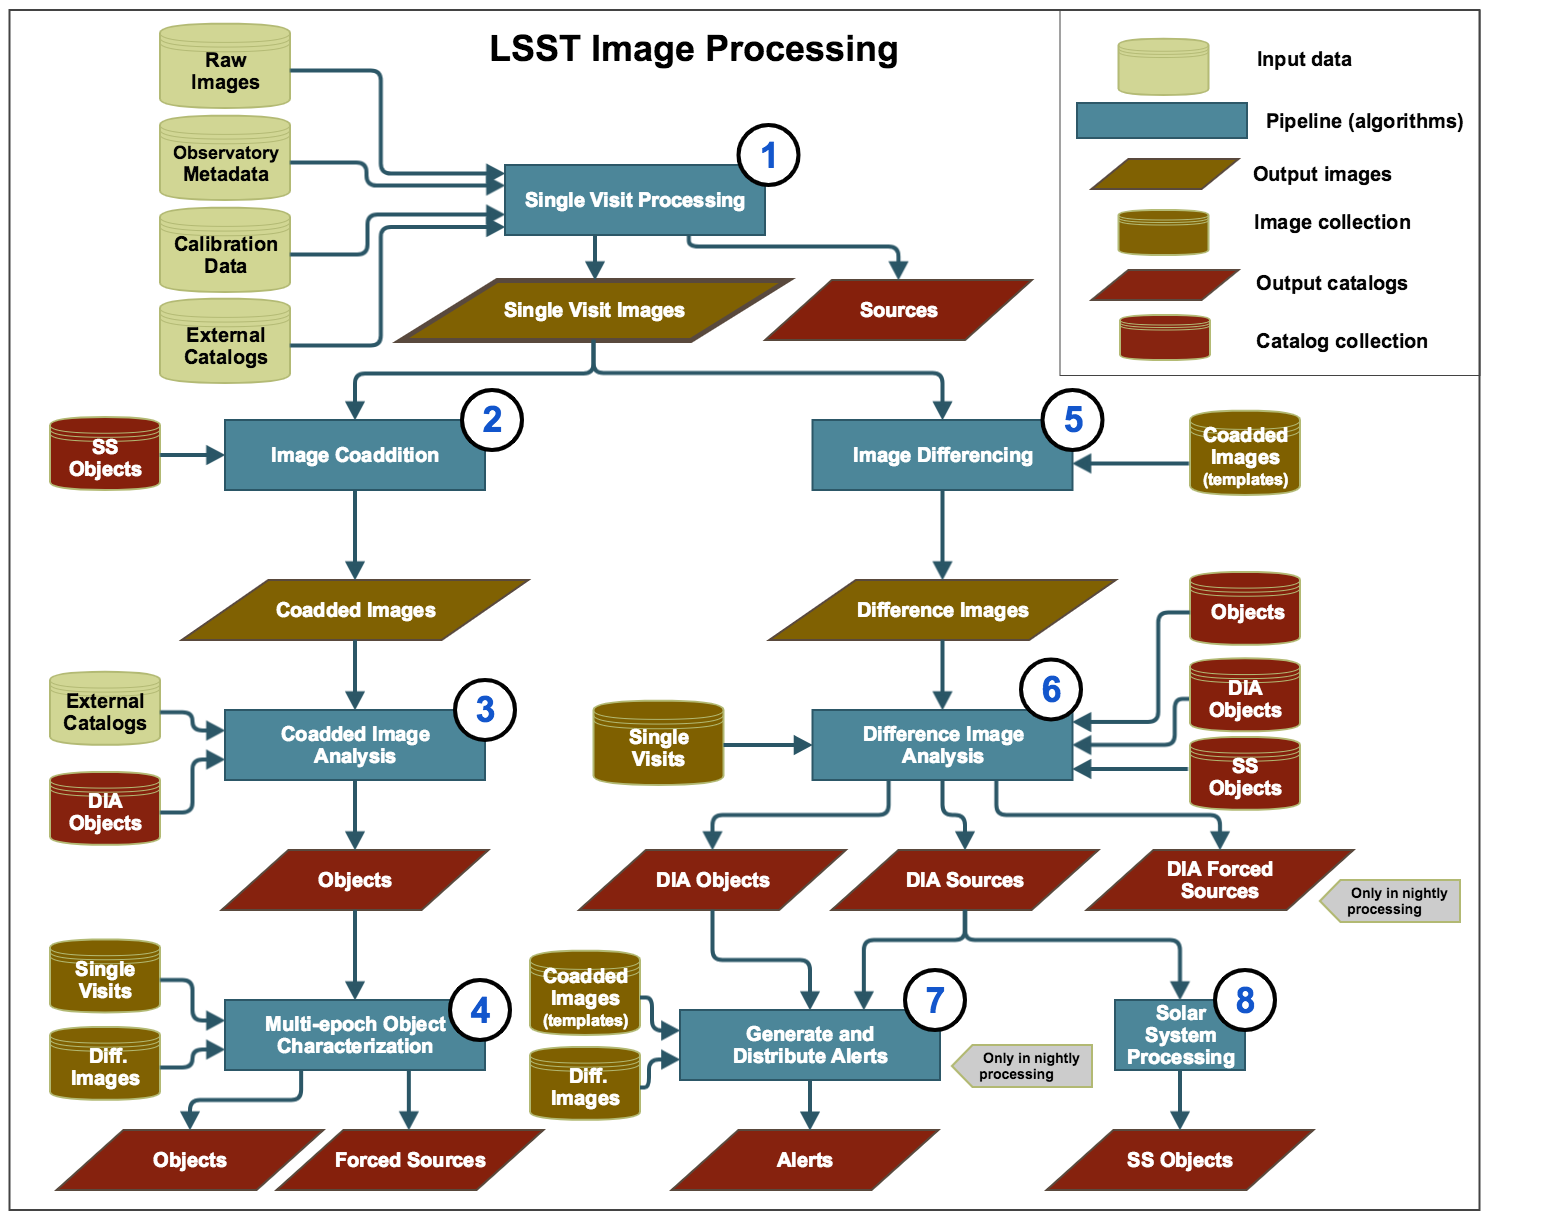
\includegraphics[scale=0.30]{gliffy/LSSTimageProcessingDetail1-v36}
    \vskip -0.1in
    \caption{Illustration of the conceptual design of LSST science pipelines for imaging processing.\label{fig:Detail1}}
\end{figure}

\begin{figure}[!t]
    \centering
    \vskip -1.1in
    \includegraphics[scale=0.505, angle=270]{gliffy/SingleVisitProcessing}
    \vskip -1.1in
    \caption{Illustration of the conceptual algorithm design for Single Visit Processing pipeline.\label{fig:Pipe1}}
\end{figure}

\begin{figure}[!th]
    \centering
    \vskip -0.2in
    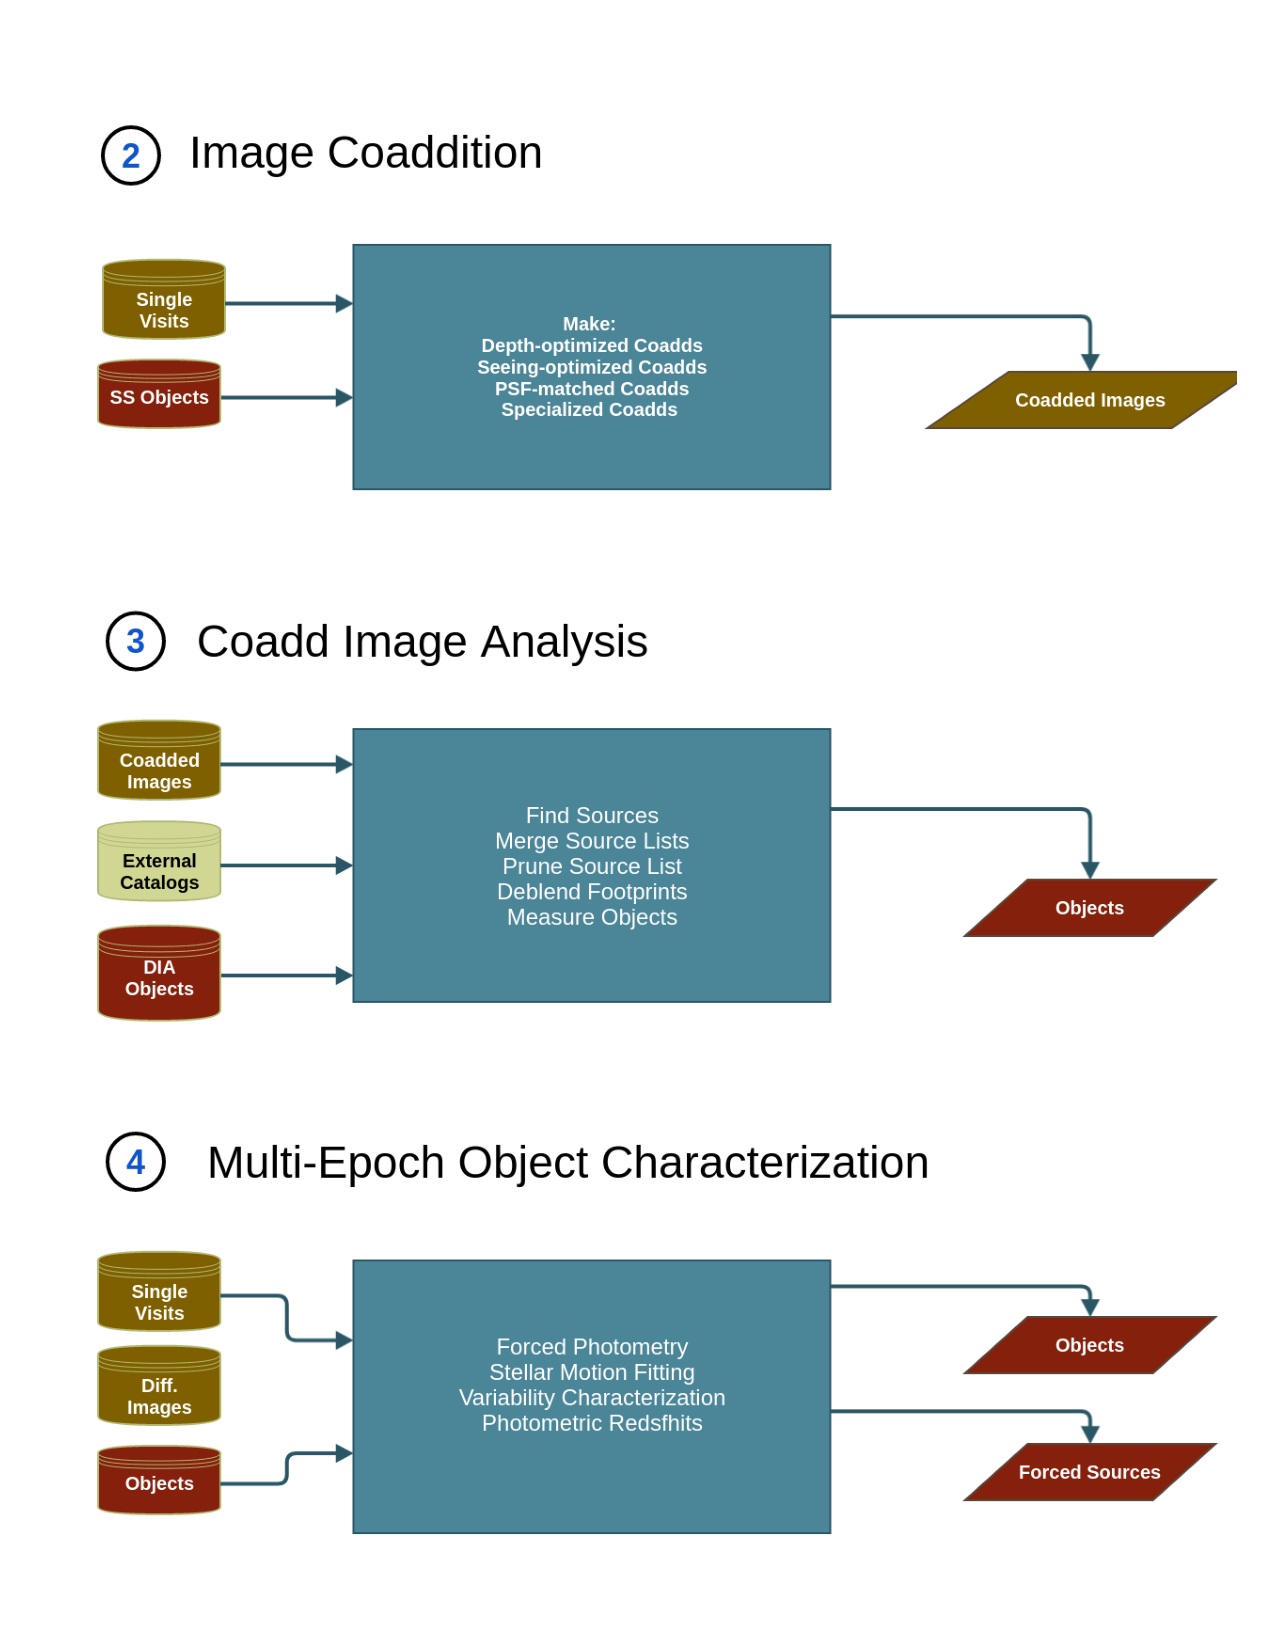
\includegraphics[scale=0.535]{gliffy/CoaddedImageProcessing}
    \vskip -0.2in
    \caption{Illustration of the conceptual algorithm design for Image Coaddition, Coadded Image Analysis,
     and Multi-epoch Object Characterization pipelines.\label{fig:Pipes234}}
\end{figure}

\begin{figure}[!th]
    \centering
    \vskip -0.3in
%    \hskip -0.8in
    \includegraphics[scale=0.555, angle=0]{gliffy/DifferenceImageProcessing}
    \vskip -0.1in
    \caption{Illustration of the conceptual algorithm  design for Image Differencing, Difference Image
                      Analysis, and Alert Generation and Distribution pipelines. \label{fig:Pipes567}}
\end{figure}

\begin{figure}[!t]
    \centering
    \vskip -0.2in
    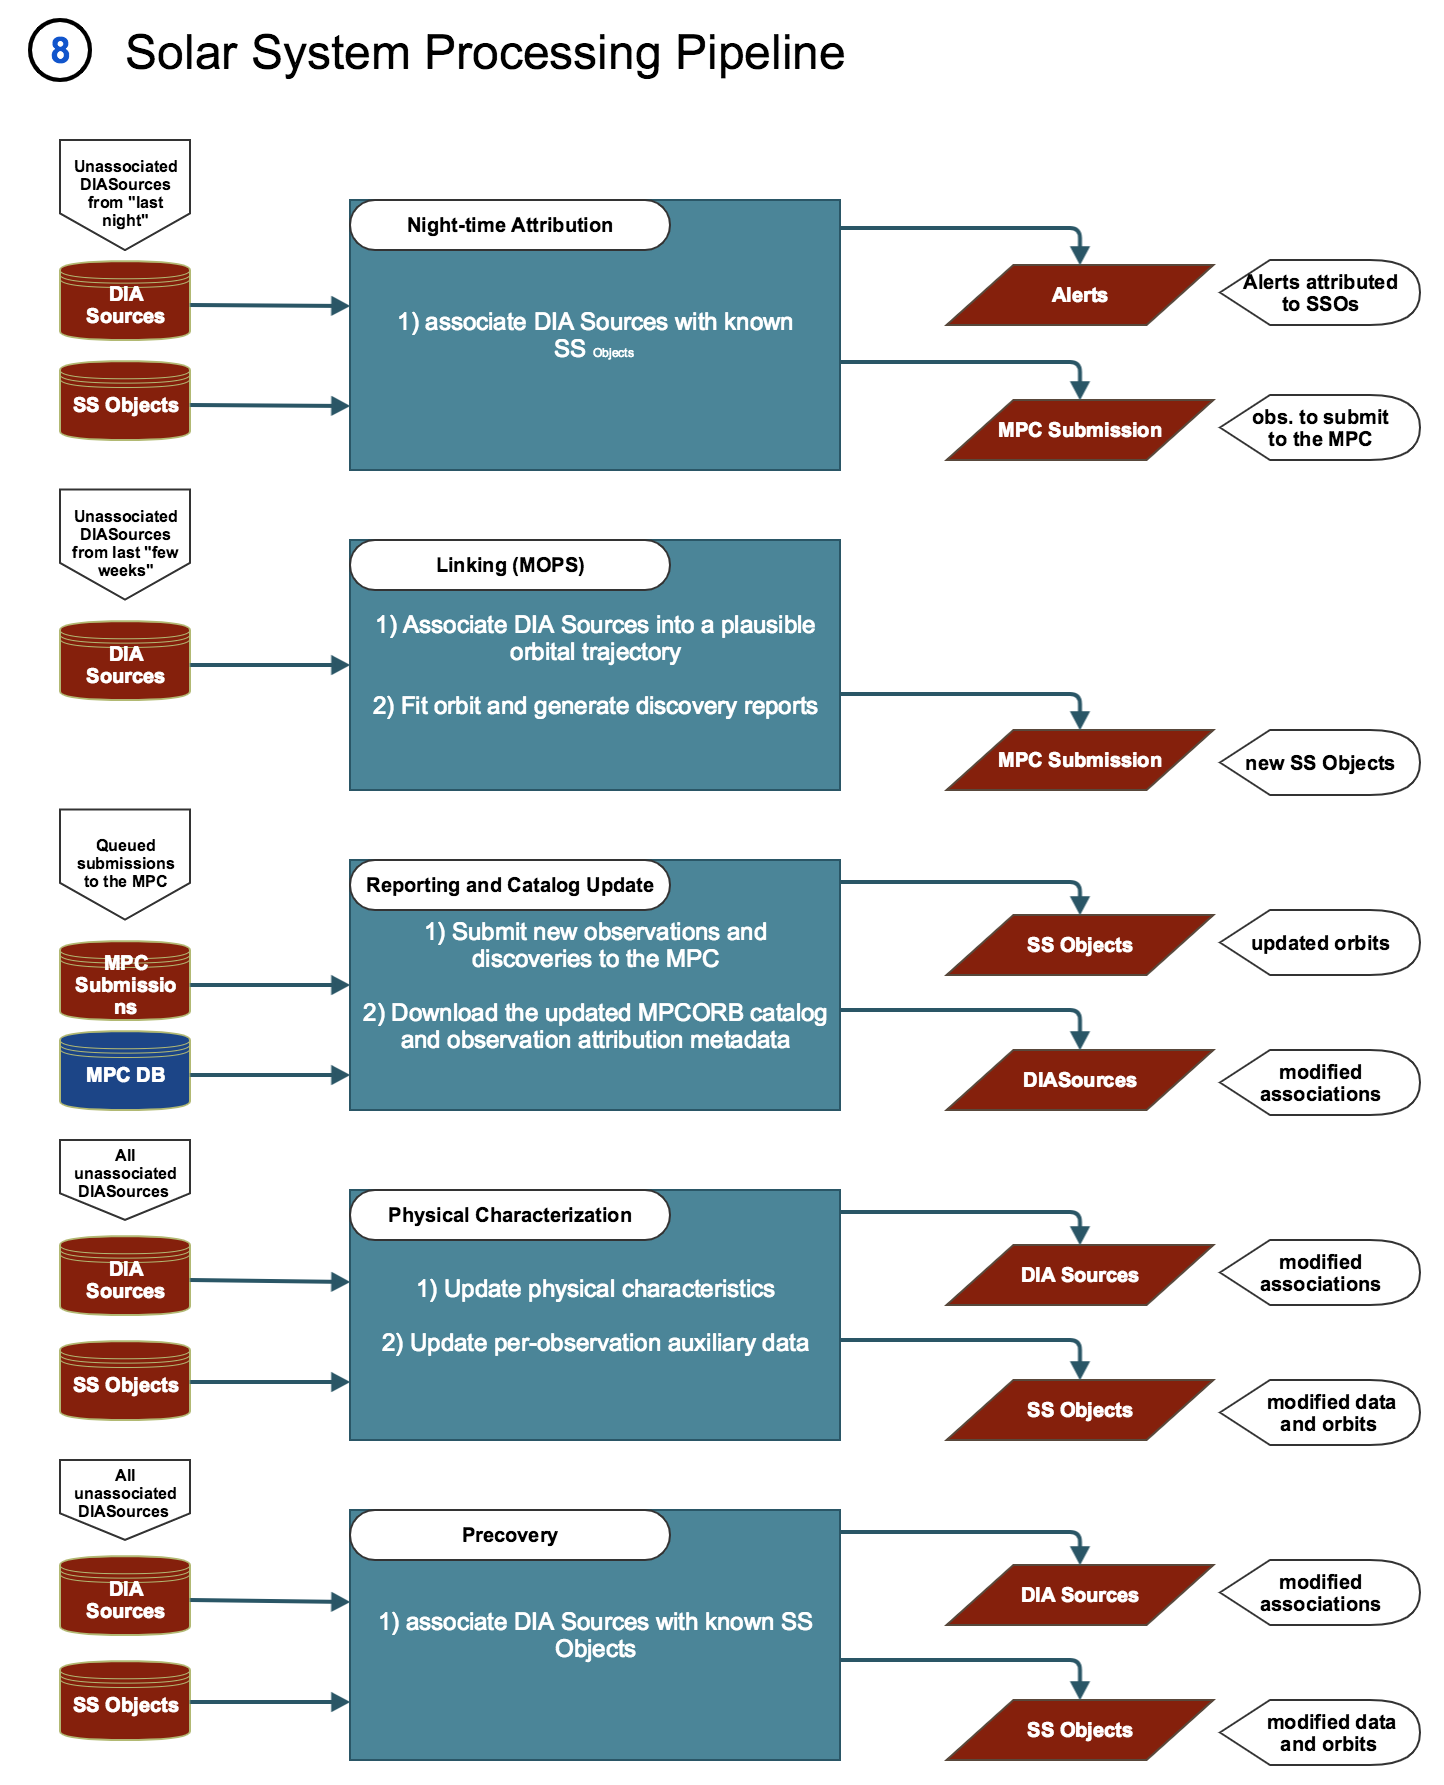
\includegraphics[scale=0.30]{gliffy/SSP-Level0-v22}
    \vskip -0.1in
    \caption{Illustration of the conceptual algorithm design for the Solar System Processing pipeline. The elements in blue denote ingestion of data from external sources.\label{fig:Pipe8}}
\end{figure}